% =====================================================================
%  BÁO CÁO TIẾN ĐỘ - Hệ thống giám sát giao thông thời gian thực tích hợp LLM (TrafficEye)
%  Nhóm Bunhen - Môn Công nghệ phần mềm
%
%  Biên dịch bằng XeLaTeX (để hiển thị tiếng Việt):
%    - Overleaf: Menu > Compiler > XeLaTeX
%    - Máy tính: xelatex main.tex (chạy 2 lần)
%  Ảnh nằm trong thư mục hinh/ (đặt cùng chỗ với file .tex). Các sơ đồ vẽ bằng TikZ ngay trong file.
% =====================================================================
\documentclass[aspectratio=169,11pt]{beamer}

\usepackage{fontspec}
\setsansfont{TeX Gyre Heros}
\usepackage{graphicx}
\usepackage{booktabs}
\usepackage{array}
\usepackage{tabularx}
\usepackage{tikz}
\usetikzlibrary{positioning,arrows.meta,fit,backgrounds,calc}

% ---------- 2 màu: đen (chữ) và xanh đậm (nhấn) ----------
\definecolor{den}{HTML}{1A1A1A}
\definecolor{mau}{HTML}{1F4E79}
\colorlet{nhat}{den!55}   % chữ phụ
\colorlet{vien}{den!25}   % đường kẻ, viền

\setbeamercolor{background canvas}{bg=white}
\setbeamercolor{normal text}{fg=den}
\setbeamercolor{frametitle}{fg=mau}
\setbeamercolor{structure}{fg=den}
\setbeamerfont{frametitle}{size=\Large,series=\bfseries}
\setbeamertemplate{navigation symbols}{}

% Gạch đầu dòng
\setbeamertemplate{itemize item}{-}
\setbeamertemplate{itemize subitem}{-}
\setlength{\leftmargini}{1.1em}

\setbeamersize{text margin left=0.9cm,text margin right=0.9cm}

% Tiêu đề slide + đường kẻ ngang bên dưới
\setbeamertemplate{frametitle}{%
  \vspace{0.5cm}%
  \begin{beamercolorbox}[wd=\paperwidth,leftskip=0.9cm]{frametitle}%
    {\usebeamerfont{frametitle}\insertframetitle}%
  \end{beamercolorbox}%
  \vspace{0.12cm}%
  {\color{vien}\rule{\dimexpr\paperwidth-1.8cm\relax}{0.5pt}}%
}

% Tên mục hiện tại, hiện ở chân trang: "Báo cáo tiến độ - <mục>"
\newcommand{\muc}{}
\newcommand{\datMuc}[1]{\renewcommand{\muc}{ - #1}}

\setbeamertemplate{footline}{%
  \hspace*{0.9cm}{\color{nhat}\scriptsize Báo cáo tiến độ\muc}%
  \hfill{\color{nhat}\scriptsize\insertframenumber/\inserttotalframenumber}\hspace*{0.9cm}%
  \vspace{0.35cm}%
}

% Tiêu đề nhỏ trong slide
\newcommand{\tieude}[1]{{\color{mau}\bfseries #1}\par\vspace{0.1cm}}

% Ảnh chụp màn hình có viền mảnh
\newcommand{\anh}[2]{{\setlength{\fboxsep}{0pt}\color{vien}\fbox{\includegraphics[#1]{#2}}}}

\begin{document}

% =====================================================================
% TRANG BÌA
% =====================================================================
{
\setbeamertemplate{footline}{}
\begin{frame}[plain]
  \begin{columns}[c,onlytextwidth]
    \column{0.6\textwidth}\raggedright
      {\color{mau}\small\bfseries BÁO CÁO TIẾN ĐỘ}\\[0.35cm]
      {\color{den}\bfseries\fontsize{20}{25}\selectfont Hệ thống giám sát\\ giao thông thời gian thực\\ tích hợp LLM\par}
      \vspace{0.2cm}
      {\color{nhat}\small TrafficEye - camera AI, bản đồ, cảnh báo sự cố, trợ lý LLM\par}
      \vspace{0.45cm}
      {\small
      \begin{tabular}{@{}l@{\hspace{0.45cm}}l@{}}
        \color{nhat}Nhóm       & bunhen \\[2pt]
        \color{nhat}Thành viên & Thái Viết Đại \\
                               & Đoàn Thanh Tuyển \\
                               & Nguyễn Thị Hà Tiên \\[2pt]
        \color{nhat}GVHD       & Đào Duy Tuấn \\[2pt]
        \color{nhat}Môn học    & Công nghệ phần mềm
      \end{tabular}}\\[0.5cm]
      {\color{nhat}\footnotesize Trường Đại học Bách khoa - Đại học Đà Nẵng \\ Tháng 11/2026}
    \column{0.38\textwidth}
      % Hình đơn giản: cột đèn tín hiệu gắn camera + màn hình giám sát
      \centering
      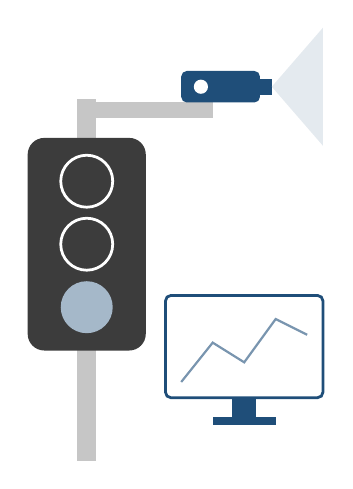
\begin{tikzpicture}
        \fill[den!25] (-0.12,-3.0) rectangle (0.12,1.6);
        \fill[den!25] (0.12,1.35) rectangle (1.6,1.55);
        \fill[mau,rounded corners=2pt] (1.2,1.55) rectangle (2.2,1.95);
        \fill[mau] (2.2,1.65) rectangle (2.35,1.85);
        \fill[white] (1.45,1.75) circle (0.09);
        \fill[mau!12] (2.35,1.75) -- (3.0,1.0) -- (3.0,2.5) -- cycle;
        \fill[den!85,rounded corners=6pt] (-0.75,-1.6) rectangle (0.75,1.1);
        \draw[white,line width=1pt] (0,0.55) circle (0.33);
        \draw[white,line width=1pt] (0,-0.25) circle (0.33);
        \fill[mau!40] (0,-1.05) circle (0.33);
        % màn hình giám sát
        \draw[mau,line width=1pt,rounded corners=2pt] (1.0,-2.2) rectangle (3.0,-0.9);
        \draw[mau!60,line width=0.8pt] (1.2,-2.0) -- (1.6,-1.5) -- (2.0,-1.75) -- (2.4,-1.2) -- (2.8,-1.4);
        \fill[mau] (1.85,-2.2) rectangle (2.15,-2.45);
        \fill[mau] (1.6,-2.45) rectangle (2.4,-2.55);
      \end{tikzpicture}
  \end{columns}
\end{frame}
}

% =====================================================================
% PHÂN CÔNG NHIỆM VỤ
% =====================================================================
% Thẻ thành viên: \thanhvien{Tên}{Vai trò}{Các dòng công việc}{Epic phụ trách}
\newcommand{\thanhvien}[4]{%
  \begin{tikzpicture}[baseline=(the.north)]
    \node[draw=vien,text width=4.15cm,minimum height=4.2cm,
          inner sep=6pt,anchor=north west,align=left] (the) at (0,0) {};
    \node[anchor=north west,text=den,font=\small\bfseries] at ($(the.north west)+(0.2,-0.2)$) {#1};
    \node[anchor=north west,text=nhat,font=\scriptsize] at ($(the.north west)+(0.2,-0.62)$) {#2};
    \draw[vien] ($(the.north west)+(0.2,-1.15)$) -- ($(the.north east)+(-0.2,-1.15)$);
    \node[anchor=north west,text width=3.95cm,align=left,font=\scriptsize] at ($(the.north west)+(0.12,-1.3)$)
      {\begin{itemize}\setlength{\itemsep}{3pt}#3\end{itemize}};
    \node[anchor=south west,font=\scriptsize,color=nhat] at ($(the.south west)+(0.2,0.15)$) {Epic: #4};
  \end{tikzpicture}}

\begin{frame}{Phân công nhiệm vụ}
  \centering
  \thanhvien{Nguyễn Thị Hà Tiên}{Nhóm trưởng}
    {\item AI Vision: YOLO11, ByteTrack
     \item Phát hiện sự cố tự động
     \item Đặc tả, UML, kiểm thử
     \item Quản lý tiến độ Sprint}
    {E03, E04}\hfill
  \thanhvien{Đoàn Thanh Tuyển}{Giao diện}
    {\item Giao diện React, bản đồ
     \item Mô phỏng camera nút giao
     \item Thống kê, biểu đồ
     \item Giao diện trợ lý AI}
    {E02, E06}\hfill
  \thanhvien{Thái Viết Đại}{Kiến trúc, máy chủ}
    {\item Kiến trúc, API FastAPI
     \item PostgreSQL, WebSocket
     \item Tích hợp LLM
     \item Docker, triển khai}
    {E01, E05, E07}\\[0.45cm]
  {\scriptsize\color{nhat}Cả nhóm cùng họp Sprint, review mã nguồn và kiểm thử}
\end{frame}

% =====================================================================
% NỘI DUNG
% =====================================================================
\begin{frame}{Nội dung}
  \vspace{0.1cm}
  \renewcommand{\arraystretch}{2}
  \begin{tabular}{@{}>{\color{mau}\bfseries}l@{\hspace{0.6cm}}>{\bfseries}l@{\hspace{1cm}}l@{}}
    1 & Tổng quan & Bài toán, mục tiêu, User Story\\
    2 & Thiết kế  & Kiến trúc, luồng AI Vision - LLM, sơ đồ UML, CSDL\\
    3 & Kết quả   & Kết quả đạt được, giao diện, AI Vision, kiểm thử\\
    4 & Tiến độ   & Tiến độ theo Epic, khó khăn\\
    5 & Kế hoạch  & Công việc tiếp theo\\
  \end{tabular}
\end{frame}

% =====================================================================
% 1. TỔNG QUAN
% =====================================================================
\datMuc{Tổng quan}

\begin{frame}{Bài toán và mục tiêu}
  \begin{columns}[c,onlytextwidth]
    \column{0.5\textwidth}
      \tieude{Bài toán}
      \begin{itemize}\footnotesize
        \item Trung tâm điều hành phải xem nhiều camera bằng mắt
        \item Phát hiện ùn tắc, tai nạn chậm, phụ thuộc người trực
        \item Số liệu lưu lượng không được ghi lại để phân tích
        \item Báo cáo tình hình phải tổng hợp thủ công
      \end{itemize}
      \vspace{0.15cm}
      \tieude{Mục tiêu}
      \begin{itemize}\footnotesize
        \item Camera AI tự nhận diện, đếm xe, đo tốc độ, mật độ
        \item Hiển thị thời gian thực trên bản đồ và dashboard
        \item Tự phát hiện sự cố, xử lý theo quy trình
        \item Trợ lý LLM tóm tắt, phân tích, đề xuất bằng tiếng Việt
      \end{itemize}
    \column{0.46\textwidth}
      \centering
      \begin{tikzpicture}[font=\scriptsize,x=1.07cm]
        \node[anchor=west,font=\small] at (0,3.05) {Giám sát thủ công};
        \fill[mau!30] (0,2.1) rectangle (6,2.7);
        \node at (3,2.4) {Người trực xem 8 màn hình camera};
        \node[anchor=west,color=nhat] at (0,1.8) {Phát hiện sự cố: vài phút, dễ bỏ sót};
        \node[anchor=west,font=\small] at (0,0.95) {Giám sát với TrafficEye};
        \fill[mau] (0,0) rectangle (2,0.6);
        \fill[mau!60] (2,0) rectangle (4,0.6);
        \fill[mau!30] (4,0) rectangle (6,0.6);
        \node[white] at (1,0.3) {AI đếm xe};
        \node[white] at (3,0.3) {Cảnh báo};
        \node at (5,0.3) {LLM đề xuất};
        \node[anchor=west,color=nhat] at (0,-0.3) {Số liệu cập nhật mỗi 2 giây, cảnh báo tức thời};
      \end{tikzpicture}\\[0.2cm]
      {\scriptsize\color{nhat}Ví dụ minh hoạ cho 8 nút giao tại Đà Nẵng}
  \end{columns}
\end{frame}

\begin{frame}{User Story}
  \centering\vspace*{-0.15cm}
  \begin{tikzpicture}[font=\scriptsize,y=0.92cm,
      cot/.style={align=center,minimum height=0.55cm,inner sep=2pt,anchor=north west,rounded corners=2pt},
      epic/.style={fill=mau!10,draw=mau!50,align=center,text width=2.2cm,minimum height=1.5cm,inner sep=3pt,anchor=north west,rounded corners=2pt},
      us/.style={fill=den!3,draw=vien,align=center,text width=6.1cm,minimum height=1.5cm,inner sep=4pt,anchor=north west,rounded corners=2pt},
      task/.style={fill=mau!5,draw=mau!35,align=left,text width=2.5cm,minimum height=0.33cm,inner sep=1.5pt,font=\tiny,anchor=north west,rounded corners=1.5pt}]
    \node[fill=mau,text=white,align=center,minimum width=1.9cm,minimum height=5.42cm,anchor=north west,rounded corners=2pt,font=\small] at (0,0) {Product\\Backlog};
    \node[cot,fill=mau!25,draw=mau!50,minimum width=2.4cm,font=\small] at (2.2,0)  {Epic};
    \node[cot,fill=den!10,draw=vien,minimum width=6.38cm,font=\small]   at (4.75,0)  {User Story};
    \node[cot,fill=mau!25,draw=mau!50,minimum width=2.6cm,font=\small] at (11.25,0) {Tasks};
    % Hàng 1: Quản trị viên
    \node[epic] at (2.2,-0.85) {E07\\Cấu hình hệ thống};
    \node[us]   at (4.75,-0.85) {\footnotesize Với vai trò là \textcolor{mau}{Quản trị viên}, tôi muốn chỉnh ngưỡng phân loại ùn tắc để hệ thống đánh giá đúng với từng tuyến đường};
    \node[task] at (11.25,-0.85) {T01 API cài đặt};
    \node[task] at (11.25,-1.24) {T02 Kiểm tra hợp lệ};
    \node[task] at (11.25,-1.63) {T03 Áp dụng ngay};
    \node[task] at (11.25,-2.02) {T04 Giao diện cài đặt};
    % Hàng 2: Điều hành viên
    \node[epic] at (2.2,-2.55) {E04\\Sự cố, cảnh báo};
    \node[us]   at (4.75,-2.55) {\footnotesize Với vai trò là \textcolor{mau}{Điều hành viên}, tôi muốn tiếp nhận và cập nhật trạng thái sự cố để mọi người thấy sự cố đang được xử lý};
    \node[task] at (11.25,-2.55) {T01 Máy trạng thái};
    \node[task] at (11.25,-2.94) {T02 Khoá dòng đồng thời};
    \node[task] at (11.25,-3.33) {T03 Phát qua WebSocket};
    \node[task] at (11.25,-3.72) {T04 Lịch sử xử lý};
    % Hàng 3: Lãnh đạo
    \node[epic] at (2.2,-4.25) {E05\\Trợ lý LLM};
    \node[us]   at (4.75,-4.25) {\footnotesize Với vai trò là \textcolor{mau}{Lãnh đạo}, tôi muốn hỏi bằng tiếng Việt "chỗ nào đang ùn tắc?" để nắm tình hình nhanh mà không cần đọc bảng số liệu};
    \node[task] at (11.25,-4.25) {T01 Dựng ngữ cảnh};
    \node[task] at (11.25,-4.64) {T02 Trả lời streaming};
    \node[task] at (11.25,-5.03) {T03 Bộ trả lời dự phòng};
    \node[task] at (11.25,-5.42) {T04 Giới hạn tần suất};
  \end{tikzpicture}\\[0.1cm]
  {\scriptsize\color{nhat}7 Epic, 16 User Story; ví dụ cho 3 vai trò: quản trị viên, điều hành viên, lãnh đạo (người xem)}
\end{frame}

% =====================================================================
% 2. THIẾT KẾ
% =====================================================================
\datMuc{Thiết kế}

\begin{frame}{Sơ đồ tổng quan hệ thống}
  \begin{columns}[c,onlytextwidth]
    \column{0.68\textwidth}
      \centering
      \begin{tikzpicture}[font=\scriptsize,
          k/.style={draw=mau!70,align=center,text width=2.1cm,minimum height=0.95cm,inner sep=3pt,rounded corners=2pt},
          n/.style={draw=vien,align=center,text width=2.1cm,minimum height=0.95cm,inner sep=3pt,rounded corners=2pt},
          mui/.style={-{Stealth[length=2mm]},thick,color=nhat},
          nhan/.style={font=\tiny,color=nhat,fill=white,inner sep=1pt}]
        \node[n] (cam) at (0,2.2)   {Camera\\(video, RTSP)};
        \node[k] (vis) at (0,0.4)   {AI Vision\\YOLO11 + ByteTrack};
        \node[n] (sim) at (0,-1.4)  {Bộ giả lập\\(khi chưa có camera)};
        \node[k,fill=mau,text=white,minimum height=3.4cm,text width=2.3cm] (be) at (3.4,0.4) {Máy chủ\\FastAPI\\[4pt]\tiny Ingest, xác thực,\\sự cố, báo cáo,\\EventBus};
        \node[n] (db)  at (6.8,2.2)  {PostgreSQL 17};
        \node[n] (llm) at (6.8,0.4)  {LLM\\Claude};
        \node[n] (fe)  at (6.8,-1.4) {Giao diện web\\React};
        \node[font=\scriptsize,color=nhat] (nd) at (6.8,-2.6) {3 vai trò người dùng};
        \draw[mui] (cam) -- (vis);
        \draw[mui] (vis) -- node[nhan,above]{số liệu, sự cố} (be.west |- vis);
        \draw[mui] (vis.east) ++(0,-0.25) -- node[nhan,below]{ảnh nhận diện} ($(be.west |- vis)+(0,-0.25)$);
        \draw[mui] (sim) -| ($(be.west)+(-0.35,-1.1)$) -- ($(be.west)+(0,-1.1)$);
        \draw[mui,{Stealth[length=2mm]}-{Stealth[length=2mm]}] (be.east |- db) -- (db.west);
        \draw[mui,{Stealth[length=2mm]}-{Stealth[length=2mm]}] (be.east |- llm) -- node[nhan,above]{chỉ số liệu} (llm.west);
        \draw[mui,{Stealth[length=2mm]}-{Stealth[length=2mm]}] (be.east |- fe) -- node[nhan,above]{REST, WS} (fe.west);
        \draw[mui] (nd) -- (fe);
      \end{tikzpicture}
    \column{0.29\textwidth}
      \begin{itemize}\footnotesize
        \item Worker AI Vision đọc video, nhận diện và đếm xe
        \item Gửi số liệu mỗi 10 s, sự cố, ảnh đã nhận diện
        \item Máy chủ lưu PostgreSQL, phát trực tiếp qua WebSocket
        \item LLM chỉ nhận số liệu tổng hợp, không nhận hình ảnh
        \item Chưa có camera thật: bộ giả lập đi qua cùng đường ống
      \end{itemize}
  \end{columns}
\end{frame}

\begin{frame}{Kiến trúc phần mềm}
  \centering
  \begin{tikzpicture}[
      font=\scriptsize,
      hop/.style={draw=vien,align=center,inner sep=4pt},
      mod/.style={draw=mau!70,align=center,inner sep=3pt,text width=2.5cm,minimum height=0.85cm},
      mui/.style={-{Stealth[length=2mm]},thick,color=nhat}]
    \node[hop,text width=1.7cm,minimum height=3.3cm] (nd) at (-0.4,0)
      {{\footnotesize\color{mau}Người dùng}\\[4pt]3 vai trò};
    \node[hop,text width=1.8cm,minimum height=3.3cm] (fe) at (2.0,0)
      {{\footnotesize\color{mau}Giao diện web}\\[4pt]React, Vite\\Leaflet};
    \node[mod] (api)  at (5.2, 1.05) {API: REST, WebSocket};
    \node[mod] (core) at (5.2, 0.0)  {Xác thực JWT, phân quyền};
    \node[mod] (svc)  at (5.2,-1.05) {Sự cố, thống kê};
    \node[mod] (vis)  at (8.0, 1.05) {Ingest số liệu, EventBus};
    \node[mod] (ctl)  at (8.0, 0.0)  {Bộ giả lập nút giao};
    \node[mod] (llm)  at (8.0,-1.05) {Dịch vụ LLM};
    \begin{scope}[on background layer]
      \node[draw=mau!40,fit=(api)(llm)(vis)(svc),inner sep=6pt,label={[font=\footnotesize,color=mau]above:Máy chủ (FastAPI)}] (be) {};
    \end{scope}
    \node[hop,text width=2.3cm,minimum height=0.8cm] (db)   at (11.5, 1.05) {Cơ sở dữ liệu\\PostgreSQL 17};
    \node[hop,text width=2.3cm,minimum height=0.8cm] (sim)  at (11.5, 0.0)  {Worker AI Vision\\YOLO11 + ByteTrack};
    \node[hop,text width=2.3cm,minimum height=0.8cm] (llmx) at (11.5,-1.05) {LLM: Claude\\claude-opus-5-5};
    \draw[mui] (nd.east) -- (fe.west);
    \draw[mui,{Stealth[length=2mm]}-{Stealth[length=2mm]}] (fe.east) -- (be.west |- fe.east);
    \draw[mui,{Stealth[length=2mm]}-{Stealth[length=2mm]}] (be.east |- db) -- (db.west);
    \draw[mui,{Stealth[length=2mm]}-{Stealth[length=2mm]}] (be.east |- sim) -- (sim.west);
    \draw[mui,{Stealth[length=2mm]}-{Stealth[length=2mm]}] (be.east |- llmx) -- (llmx.west);
  \end{tikzpicture}
  \vspace{0.15cm}
  \raggedright
  \begin{itemize}\footnotesize
    \item Kiến trúc phân tầng: router - service - repository - domain; mẫu Observer (EventBus), Adapter, Strategy
    \item Giao diện gửi yêu cầu qua REST, nhận dữ liệu trực tiếp qua WebSocket (có xác thực JWT)
    \item Lược đồ CSDL quản lý phiên bản bằng Alembic; chạy toàn bộ bằng Docker Compose
  \end{itemize}
\end{frame}

\begin{frame}{Từ video đến LLM: 3 tầng xử lý}
  \begin{columns}[c,onlytextwidth]
    \column{0.64\textwidth}
    \begin{tikzpicture}[font=\footnotesize,
        tang/.style={fill=mau,text=white,align=center,text width=2.3cm,minimum height=1.3cm,inner sep=3pt},
        mota/.style={draw=mau!60,align=left,text width=5.0cm,minimum height=1.3cm,inner sep=5pt,anchor=west},
        mui/.style={-{Stealth[length=2.2mm]},thick,color=nhat}]
      \node[tang] (t1) at (0,2.1)  {Tầng 1\\YOLO11 + ByteTrack};
      \node[tang] (t2) at (0,0)    {Tầng 2\\Thống kê (Python)};
      \node[tang] (t3) at (0,-2.1) {Tầng 3\\LLM diễn giải};
      \node[mota] (m1) at ($(t1.east)+(0.3,0)$) {Nhận diện, gán ID, đếm xe cắt vạch; đo tốc độ, chiếm dụng làn\\{\color{nhat}mỗi khung hình, gửi số liệu mỗi 10 s}};
      \node[mota] (m2) at ($(t2.east)+(0.3,0)$) {Xu hướng, đỉnh, bất thường (lệch 2 độ lệch chuẩn), dự báo 15 phút\\{\color{nhat}tính chính xác, có kiểm thử}};
      \node[mota] (m3) at ($(t3.east)+(0.3,0)$) {Đọc các con số đã tính, giải thích và đề xuất điều hành\\{\color{nhat}khi người dùng yêu cầu}};
      \draw[mui] (t1.south) -- node[left,font=\scriptsize,color=nhat]{số liệu} (t2.north);
      \draw[mui] (t2.south) -- node[left,font=\scriptsize,color=nhat]{thống kê} (t3.north);
    \end{tikzpicture}
    \column{0.33\textwidth}
      \tieude{Nguyên tắc}
      \begin{itemize}\footnotesize
        \item LLM không tự tính số, chỉ diễn giải số liệu đã tính
        \item LLM không nhận hình ảnh: rẻ hơn, không lộ biển số
        \item Ngữ cảnh luôn dựng từ dữ liệu trên máy chủ
        \item LLM lỗi hoặc chưa có khoá thì dùng bộ trả lời theo luật
        \item Giới hạn 20 yêu cầu/phút mỗi người, ghi nhật ký token
      \end{itemize}
  \end{columns}
\end{frame}

\begin{frame}{Biểu đồ trạng thái sự cố}
  \begin{columns}[c,onlytextwidth]
    \column{0.64\textwidth}
      \centering
      \begin{tikzpicture}[font=\scriptsize,
          st/.style={draw=mau!70,fill=mau!8,rounded corners=6pt,align=center,text width=2.1cm,minimum height=0.9cm},
          mui/.style={-{Stealth[length=2mm]},thick,color=nhat},
          nhan/.style={font=\tiny,color=den,fill=white,inner sep=1pt}]
        \fill[den] (-1.6,1.6) circle (0.12);
        \node[st] (new) at (0,1.6) {Mới\\\tiny NEW};
        \node[st] (ack) at (3.2,1.6) {Đã tiếp nhận\\\tiny ACKNOWLEDGED};
        \node[st] (inp) at (6.4,1.6) {Đang xử lý\\\tiny IN\_PROGRESS};
        \node[st] (res) at (6.4,-0.9) {Đã xử lý\\\tiny RESOLVED};
        \node[st] (fal) at (1.6,-0.9) {Báo động giả\\\tiny FALSE\_ALARM};
        \draw[mui] (-1.48,1.6) -- node[nhan,above]{AI phát hiện} (new);
        \draw[mui] (new) -- node[nhan,above]{tiếp nhận} (ack);
        \draw[mui] (ack) -- node[nhan,above]{bắt đầu} (inp);
        \draw[mui] (inp) -- node[nhan,right]{hoàn tất} (res);
        \draw[mui] (new.south) -- node[nhan,left]{báo động giả} (fal.north west);
        \draw[mui] (ack.south) -- (fal.north east);
        \draw[mui] (inp.south west) -- (fal.east);
        \draw[mui,dashed] (res.south) -- ++(0,-0.6) -| node[nhan,pos=0.25,below]{mở lại} (fal.south);
        \draw[mui,dashed] (fal.west) -| node[nhan,pos=0.7,left]{mở lại} (new.west);
      \end{tikzpicture}
    \column{0.33\textwidth}
      \begin{itemize}\footnotesize
        \item Cùng một máy trạng thái ở giao diện và máy chủ
        \item Không cho bỏ bước: Mới sang Đã xử lý bị từ chối (409)
        \item Người xem không có quyền xử lý (403)
        \item Hai người cùng bấm: khoá dòng \texttt{SELECT ... FOR UPDATE}
        \item Mỗi bước ghi lịch sử: người làm, thời điểm, ghi chú
      \end{itemize}
  \end{columns}
\end{frame}

\begin{frame}{Biểu đồ tuần tự: từ camera đến phân tích LLM}
  \centering
  \resizebox{\linewidth}{!}{%
  \begin{tikzpicture}[font=\scriptsize,y=0.62cm,
      ben/.style={draw=mau!70,fill=mau!8,align=center,text width=2.1cm,minimum height=0.7cm,inner sep=2pt},
      msg/.style={-{Stealth[length=1.8mm]},color=den},
      ret/.style={-{Stealth[length=1.8mm]},dashed,color=nhat},
      t/.style={font=\tiny,fill=white,inner sep=1pt}]
    \foreach \x/\n/\l in {0/w/Worker AI Vision,3/b/Máy chủ FastAPI,6/d/PostgreSQL,9/f/Trình duyệt,12/l/LLM}{
      \node[ben] (\n) at (\x,0) {\l};
      \draw[vien,dashed] (\x,-0.6) -- (\x,-9.6);
    }
    \draw[msg] (0,-1.3) -- node[t,above]{POST /ingest/metrics (mỗi 10 s)} (3,-1.3);
    \draw[msg] (3,-2.1) -- node[t,above]{lưu số liệu} (6,-2.1);
    \draw[msg] (3,-2.9) -- node[t,above,pos=0.75]{WS metrics:update} (9,-2.9);
    \draw[msg] (0,-3.7) -- node[t,above]{POST /ingest/frames (1 ảnh/s)} (3,-3.7);
    \draw[msg] (3,-4.5) -- node[t,above,pos=0.75]{WS camera:frame} (9,-4.5);
    \draw[msg] (9,-5.5) -- node[t,above,pos=0.3]{POST /llm/analyze-traffic} (3,-5.5);
    \draw[msg] (3,-6.3) -- node[t,above]{chuỗi số liệu theo phút} (6,-6.3);
    \draw[msg] (3,-7.0) -- ++(0.6,0) -- ++(0,-0.45) -- node[t,below]{tính thống kê} ++(-0.6,0);
    \draw[msg] (3,-8.2) -- node[t,above,pos=0.75]{số liệu + thống kê} (12,-8.2);
    \draw[ret] (12,-8.8) -- node[t,above,pos=0.25]{phân tích có cấu trúc} (3,-8.8);
    \draw[ret] (3,-9.4) -- node[t,above]{kết quả hiển thị} (9,-9.4);
  \end{tikzpicture}}
\end{frame}

\begin{frame}{Thiết kế cơ sở dữ liệu}
  \begin{columns}[c,onlytextwidth]
    \column{0.66\textwidth}
      \centering
      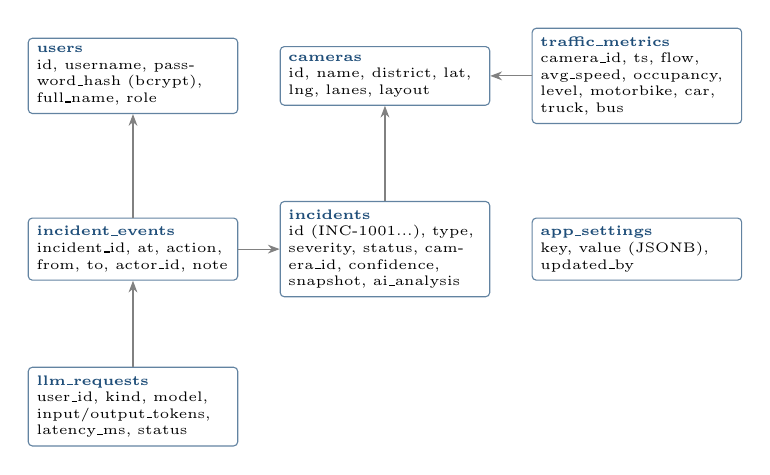
\begin{tikzpicture}[font=\tiny,
          bang/.style={draw=mau!70,align=left,text width=2.45cm,inner sep=3pt,rounded corners=1.5pt},
          lk/.style={-{Stealth[length=1.5mm]},color=nhat}]
        \node[bang] (u) at (0,2.2) {\textbf{\color{mau}users}\\id, username, password\_hash (bcrypt), full\_name, role};
        \node[bang] (c) at (3.2,2.2) {\textbf{\color{mau}cameras}\\id, name, district, lat, lng, lanes, layout};
        \node[bang] (m) at (6.4,2.2) {\textbf{\color{mau}traffic\_metrics}\\camera\_id, ts, flow, avg\_speed, occupancy, level, motorbike, car, truck, bus};
        \node[bang] (i) at (3.2,0.0) {\textbf{\color{mau}incidents}\\id (INC-1001...), type, severity, status, camera\_id, confidence, snapshot, ai\_analysis};
        \node[bang] (e) at (0,0.0) {\textbf{\color{mau}incident\_events}\\incident\_id, at, action, from, to, actor\_id, note};
        \node[bang] (s) at (6.4,0.0) {\textbf{\color{mau}app\_settings}\\key, value (JSONB), updated\_by};
        \node[bang] (l) at (0,-2.0) {\textbf{\color{mau}llm\_requests}\\user\_id, kind, model, input/output\_tokens, latency\_ms, status};
        \draw[lk] (m.west) -- (c.east);
        \draw[lk] (i.north) -- (c.south);
        \draw[lk] (e.east) -- (i.west);
        \draw[lk] (e.north) -- (u.south);
        \draw[lk] (l.north) -- (e.south);
      \end{tikzpicture}
    \column{0.31\textwidth}
      \begin{itemize}\footnotesize
        \item PostgreSQL 17, 7 bảng nghiệp vụ
        \item Ràng buộc CHECK cho trạng thái, mức độ, mức ùn tắc
        \item Chỉ mục theo \texttt{(camera\_id, ts DESC)} cho chuỗi thời gian
        \item Số liệu chi tiết giữ 7 ngày, tự dọn mỗi giờ
        \item Kết quả phân tích LLM lưu lại, không gọi lại tốn phí
      \end{itemize}
  \end{columns}
\end{frame}

% =====================================================================
% 3. KẾT QUẢ
% =====================================================================
\datMuc{Kết quả}

\begin{frame}{Kết quả đạt được}
  \begin{columns}[T,onlytextwidth]
    \column{0.48\textwidth}
      \tieude{Người dùng và giám sát}
      \begin{itemize}\footnotesize
        \item Đăng nhập JWT, phân quyền 3 vai trò
        \item Dashboard, bản đồ, 8 camera cập nhật mỗi 2 giây
        \item Mô phỏng ngã tư có đèn và Ngã ba Huế khác mức
        \item Hình trực tiếp từ YOLO11 + ByteTrack trên giao diện
        \item Sự cố tự phát hiện, xử lý theo quy trình
      \end{itemize}
    \column{0.48\textwidth}
      \tieude{Phân tích và báo cáo}
      \begin{itemize}\footnotesize
        \item Trợ lý LLM hỏi đáp tiếng Việt, trả lời dần từng chữ
        \item LLM phân tích sự cố và phân tích lưu lượng
        \item Báo cáo theo nút giao, loại sự cố, xuất CSV
        \item Cấu hình ngưỡng ùn tắc, áp dụng ngay
        \item Tài liệu đặc tả, UML, kiến trúc, kiểm thử, Scrum
      \end{itemize}
  \end{columns}
  \vspace{0.2cm}
  \tieude{Công nghệ sử dụng}
  \footnotesize
  \renewcommand{\arraystretch}{1.3}
  \begin{tabular}{@{}l@{\hspace{0.9cm}}l@{\hspace{0.9cm}}l@{\hspace{0.9cm}}l@{\hspace{0.9cm}}l@{}}
    \toprule
    \color{nhat}Máy chủ & \color{nhat}Giao diện & \color{nhat}Cơ sở dữ liệu & \color{nhat}AI Vision & \color{nhat}LLM\\
    Python, FastAPI & React, Vite & PostgreSQL 17 & YOLO11, ByteTrack & Claude (opus-5-5)\\
    \bottomrule
  \end{tabular}
\end{frame}

\begin{frame}{Giao diện tổng quan}
  \begin{columns}[T,onlytextwidth]
    \column{0.66\textwidth}
      \anh{width=\linewidth}{hinh/tongquan.jpg}
    \column{0.31\textwidth}
      \footnotesize
      \begin{itemize}
        \item 4 chỉ số: lưu lượng, tốc độ, chỉ số ùn tắc, sự cố đang mở
        \item Biểu đồ lưu lượng và tốc độ toàn mạng theo thời gian thực
        \item Nhận định tình hình do LLM tóm tắt
        \item Cơ cấu phương tiện: xe máy, ô tô, xe tải, xe buýt
        \item Màu theo đèn giao thông: xanh, vàng, cam, đỏ
      \end{itemize}
  \end{columns}
\end{frame}

\begin{frame}{Bản đồ và mô phỏng nút giao}
  \begin{columns}[T,onlytextwidth]
    \column{0.48\textwidth}
      \anh{width=\linewidth}{hinh/bando.jpg}\\[0.1cm]
      {\color{mau}\small Bản đồ giao thông Đà Nẵng}
      \begin{itemize}\scriptsize
        \item 8 nút giao tô màu theo mức ùn tắc
        \item Ghim sự cố theo loại, bấm để xem chi tiết
      \end{itemize}
    \column{0.48\textwidth}
      \anh{width=\linewidth}{hinh/camera_ngabahue.jpg}\\[0.1cm]
      {\color{mau}\small Ngã ba Huế: nút giao khác mức}
      \begin{itemize}\scriptsize
        \item Vòng xuyến, cầu vượt, đường dẫn cong; xe nhường xe trong vòng
        \item Các nút khác: ngã tư có đèn theo pha, xe xếp hàng khi đèn đỏ
      \end{itemize}
  \end{columns}
\end{frame}

\begin{frame}{AI Vision: YOLO11 + ByteTrack chạy thật}
  \begin{columns}[T,onlytextwidth]
    \column{0.48\textwidth}
      \anh{width=\linewidth}{hinh/yolo_nhandien.jpg}\\[0.1cm]
      {\color{mau}\small Nhận diện và bám vết trên video}
      \begin{itemize}\scriptsize
        \item Khung xe, ID bám vết, độ tin cậy, vạch đếm, vùng làn
        \item Ô tô nhận diện với độ tin cậy khoảng 0,88; ID giữ ổn định
      \end{itemize}
    \column{0.48\textwidth}
      \anh{width=\linewidth}{hinh/camera_vision.jpg}\\[0.1cm]
      {\color{mau}\small Hình trực tiếp trên giao diện}
      \begin{itemize}\scriptsize
        \item Worker gửi khoảng 1 ảnh/giây, nhãn "TRỰC TIẾP"
        \item CPU: 12-16 khung hình/giây với yolo11n
      \end{itemize}
  \end{columns}
\end{frame}

\begin{frame}{Sự cố và trợ lý LLM}
  \begin{columns}[T,onlytextwidth]
    \column{0.48\textwidth}
      \anh{width=\linewidth}{hinh/suco.jpg}\\[0.1cm]
      {\color{mau}\small Xử lý sự cố}
      \begin{itemize}\scriptsize
        \item Phân tích: nguyên nhân, tác động, hành động đề xuất
        \item Nút xử lý chỉ hiện các bước hợp lệ; lịch sử xử lý
      \end{itemize}
    \column{0.48\textwidth}
      \anh{width=\linewidth}{hinh/trolyai.jpg}\\[0.1cm]
      {\color{mau}\small Trợ lý LLM điều hành}
      \begin{itemize}\scriptsize
        \item Trả lời dựa đúng số liệu thời gian thực
        \item Hiện rõ ngữ cảnh đã gửi cho AI
      \end{itemize}
  \end{columns}
\end{frame}

\begin{frame}{Phân tích lưu lượng bằng LLM}
  \begin{columns}[T,onlytextwidth]
    \column{0.62\textwidth}
      \anh{width=\linewidth}{hinh/phantich_luuluong.jpg}
    \column{0.35\textwidth}
      \footnotesize
      \begin{itemize}
        \item Chọn khoảng 15 phút, 1 giờ hoặc 3 giờ
        \item Lưu lượng TB, tốc độ TB, xu hướng, dự báo 15 phút
        \item Thời điểm cao điểm, bất thường, đề xuất điều hành
        \item Ghi rõ nguồn: AI Vision (camera thật) hay bộ giả lập
      \end{itemize}
      \vspace{0.15cm}
      {\scriptsize\color{nhat}Ảnh chụp khi chưa có khoá Claude: phần diễn giải do bộ trả lời theo luật đảm nhận}
  \end{columns}
\end{frame}

\begin{frame}{Kiểm thử}
  \begin{columns}[c,onlytextwidth]
    \column{0.55\textwidth}
      \footnotesize
      \renewcommand{\arraystretch}{1.4}
      \begin{tabular}{@{}l l r@{}}
        \toprule
        \textbf{Phần} & \textbf{Công cụ} & \textbf{Kết quả}\\
        \midrule
        Giao diện       & Vitest           & 66/66\\
        Máy chủ, unit   & pytest           & 48/48\\
        Máy chủ, tích hợp & pytest + PostgreSQL & 25/25\\
        AI Vision       & pytest           & 7/7\\
        \midrule
        \textbf{Tổng}   &                  & \textbf{146/146}\\
        \bottomrule
      \end{tabular}
    \column{0.42\textwidth}
      \tieude{Một số ca kiểm thử}
      \begin{itemize}\scriptsize
        \item Sai mật khẩu 401, không đủ quyền 403, bỏ bước 409
        \item WebSocket từ chối token sai; người xử lý lấy từ token
        \item Mô phỏng: 0 xe vượt đèn đỏ, 0 xe chồng nhau (5 seed, 3 mức lưu lượng)
        \item AI Vision: đếm mỗi xe 1 lần, phát hiện đi ngược chiều, xe dừng
        \item Chạy thử trọn luồng camera - máy chủ - LLM
      \end{itemize}
  \end{columns}
\end{frame}

% =====================================================================
% 4. TIẾN ĐỘ
% =====================================================================
\datMuc{Tiến độ}

\begin{frame}{Tiến độ theo Epic}
  \small
  \renewcommand{\arraystretch}{1.45}
  \begin{tabularx}{\textwidth}{@{}l>{\bfseries}p{3.6cm}cl>{\raggedright\arraybackslash}X@{}}
    \toprule
    \textbf{Epic} & \textbf{Nội dung} & \textbf{US xong} & \textbf{Trạng thái} & \textbf{Ghi chú}\\
    \midrule
    E01 & Người dùng, phân quyền  & 2/2 & Hoàn thành & \\
    E02 & Giám sát thời gian thực & 3/3 & Hoàn thành & \\
    E03 & AI Vision, đếm xe       & 2/3 & {\color{mau}\bfseries Đang làm} & Chưa đánh giá trên video giao thông thực tế\\
    E04 & Sự cố, cảnh báo         & 2/2 & Hoàn thành & \\
    E05 & Trợ lý LLM              & 3/3 & Hoàn thành & Chưa chạy với khoá Claude thật\\
    E06 & Thống kê, báo cáo       & 1/2 & {\color{mau}\bfseries Đang làm} & Chưa lưu trữ dài hạn theo ngày, tháng\\
    E07 & Cấu hình hệ thống       & 1/1 & Hoàn thành & \\
    \midrule
    \multicolumn{2}{@{}l}{\bfseries Tổng} & \bfseries 14/16 & & \\
    \bottomrule
  \end{tabularx}
\end{frame}

\begin{frame}{Khó khăn và cách xử lý}
  \footnotesize
  \renewcommand{\arraystretch}{1.75}
  \begin{tabularx}{\textwidth}{@{}>{\raggedright\arraybackslash}p{5.2cm}>{\raggedright\arraybackslash}X@{}}
    \toprule
    \textbf{Khó khăn} & \textbf{Cách xử lý}\\
    \midrule
    Không có camera thật tại nút giao
      & Bộ giả lập đi qua cùng đường ống ingest như dữ liệu thật; camera có AI Vision thì giả lập tự nhường\\
    Chưa có khoá API cho LLM
      & Bộ trả lời theo luật dùng chung giao diện; có khoá thì tự chuyển sang Claude\\
    Chưa có video giao thông Việt Nam để đánh giá YOLO
      & Kiểm chứng bằng video mẫu công khai; kế hoạch quay video tại nút giao Đà Nẵng, đếm tay để so sánh\\
    Ổ đĩa đầy khi cài thư viện AI (torch); Docker tự tắt
      & Cài môi trường AI sang ổ khác; đặt \texttt{restart: unless-stopped} cho CSDL\\
    Dịch vụ nền bản đồ CARTO yêu cầu khoá API
      & Chuyển sang nền OpenStreetMap, giao diện tối dùng bộ lọc màu\\
    \bottomrule
  \end{tabularx}
\end{frame}

% =====================================================================
% 5. KẾ HOẠCH
% =====================================================================
\datMuc{Kế hoạch}

\begin{frame}{Công việc tiếp theo}
  \footnotesize
  \renewcommand{\arraystretch}{1.8}
  \begin{tabularx}{\textwidth}{@{}l>{\raggedright\arraybackslash}p{5.4cm}>{\raggedright\arraybackslash}X@{}}
    \toprule
     & \textbf{Công việc} & \textbf{Kết quả cần có}\\
    \midrule
    1 & Đánh giá YOLO trên video giao thông thực tế & Sai số đếm xe so với đếm tay, hiệu chỉnh vạch đếm, mét/pixel\\
    2 & Tinh chỉnh mô hình cho xe máy Việt Nam      & Mô hình nhận diện xe máy dày đặc tốt hơn bản COCO gốc\\
    3 & Chạy LLM với khoá Claude thật               & Đánh giá chất lượng câu trả lời, chi phí token\\
    4 & Quản lý tài khoản, CI chạy kiểm thử tự động & User Story còn lại của E07, GitHub Actions\\
    5 & Hoàn thiện sản phẩm cuối kỳ                 & Báo cáo, slide, video demo\\
    \bottomrule
  \end{tabularx}
\end{frame}

\end{document}
